%% LyX 1.4.3 created this file.  For more info, see http://www.lyx.org/.
%% Do not edit unless you really know what you are doing.
\documentclass[10pt,english]{article}
\usepackage[latin1]{inputenc}
\setcounter{secnumdepth}{3}
\setcounter{tocdepth}{3}
\usepackage{graphicx}
\usepackage{amssymb}
\IfFileExists{url.sty}{\usepackage{url}}
                      {\newcommand{\url}{\texttt}}

\makeatletter

%%%%%%%%%%%%%%%%%%%%%%%%%%%%%% LyX specific LaTeX commands.
%% Bold symbol macro for standard LaTeX users
\providecommand{\boldsymbol}[1]{\mbox{\boldmath $#1$}}

%% A simple dot to overcome graphicx limitations
\newcommand{\lyxdot}{.}


%%%%%%%%%%%%%%%%%%%%%%%%%%%%%% Textclass specific LaTeX commands.
 \usepackage{icml2007}
 \usepackage{mlapa}
 \usepackage{epsf}
 \usepackage{amsmath}
 \usepackage{amsthm}
 \usepackage{amsfonts}

%%%%%%%%%%%%%%%%%%%%%%%%%%%%%% User specified LaTeX commands.
\usepackage{subfigure}
\usepackage{graphicx}
\usepackage{mlapa}

\usepackage{babel}
\makeatother
\begin{document}
\twocolumn[

\icmltitle{Hierarchical Gaussian Process Latent Variable Models}

\icmlauthor{Neil D. Lawrence}{neill@cs.man.ac.uk}
\icmladdress{School of Computer Science, University of Manchester, Kilburn Building, Oxford Road, Manchester, M13 9PL, U.K.}

\icmlauthor{Andrew J. Moore}{A.Moore@dcs.shef.ac.uk}

\icmladdress{Dept of Computer Science, University of Sheffield, Regent Court, 211 Portobello Street, Sheffield, S1 4DP, U.K.}
]

\begin{abstract}
The Gaussian process latent variable model (GP-LVM) is a powerful
approach for probabilistic modelling of high dimensional data through
dimensional reduction. In this paper we extend the GP-LVM through
hierarchies. A hierarchical model (such as a tree) allows us to express
conditional independencies in the data as well as the manifold structure.
We first introduce Gaussian process hierarchies through a simple dynamical
model, we then extend the approach to a more complex hierarchy which
is applied to the visualisation of human motion data sets.
\end{abstract}

\section{Introduction}

The Gaussian process latent variable model \cite{Lawrence:gplvm03,Lawrence:pnpca05}
has proven to be a highly effective approach to probabilistic modelling
of high dimensional data that lies on a non-linear manifold \cite{Grochow:styleik04,Urtasun:priors05,Urtasun:3dpeople06,Ferris:wifi07}.
The curse of dimensionality is finessed by assuming that the high
dimensional data is intrinsically low dimensional in nature. This
reduces the effective number of parameters in the model enabling good
generalisation from very small data sets using non-linear models (even
when the dimensionality of the features, $d$, is larger than the
number of data points, $N$).

One alternative to manifold representations when modelling high dimensional
data is to develop a latent variable model with sparse connectivity
to explain the data. For example tree structured models have been
suggested for modelling images \cite{Williams:tree98,Feng:combining02,Awasthi:image07},
for object recognition \cite{Felzenszwalb:efficient00,Ioffe:mixtures01}
and human pose estimation \cite{Ramanan:finding03,Sigal:loose04,Lan:beyond05}.
From the probabilistic perspective \cite{Pearl:book88} the tree structures
(and other sparse probabilistic models) offer a convenient way to
specify conditional independencies in the model. In general, it is
not clear how such conditional independencies can be specified within
the context of dimensional reduction. In this paper we will show how
we can construct our dimensionality reduction in a hierarchical way
allowing us to concurrently exploit the advantages of expressing conditional
independencies and low dimensional non-linear manifolds.


\subsection{GP-LVMs}

The Gaussian process latent variable model (GP-LVM) is a fully probabilistic,
non-linear, latent variable model that generalises principal component
analysis. The model was inspired by the observation that a particular
probabilistic interpretation of PCA is a product of Gaussian process
models each with a \emph{linear} covariance function. Through consideration
of non-linear covariance functions a non-linear latent variable model
can be constructed \cite{Lawrence:gplvm03,Lawrence:pnpca05}.

An important characteristic of the GP-LVM is the ease and accuracy
with which probabilistic reconstructions of the data can be made,
given a (possibly new) point in the latent space. This characteristic
is exploited in several of the successful applications of the GP-LVM:
learning style from motion capture data \cite{Grochow:styleik04}
learning a prior model for tracking \cite{Urtasun:priors05,Urtasun:3dpeople06}
and robot simultaneous localisation and mapping \cite{Ferris:wifi07}.
All make use of smooth mappings from the latent space to the data
space.

The probabilistic approach to non-linear dimensionality reduction
\cite{MacKay:wondsa95,Bishop:gtm_ncomp98} is to formulate a latent
variable model, where the latent dimension, $q$, is lower than the
data dimension, $d$. The latent space is then governed by a prior
distribution $p\left(\mathbf{X}\right)$. The latent variable is related
to the observation space through a probabilistic mapping,\[
y_{ni}=f_{i}\left(\mathbf{x}_{n};\mathbf{W}\right)+\epsilon_{n},\]
 where $y_{ni}$ is the $i$th feature of the $n$th data point and
$\epsilon_{n}$ is a noise term that is typically taken to be Gaussian%
\footnote{We denote a Gaussian distribution over $\mathbf{z}$ with mean $\boldsymbol{\mu}$
and covariance $\boldsymbol{\Sigma}$ by $N\left(\mathbf{z}|\boldsymbol{\mu,\boldsymbol{\Sigma}}\right)$.%
}, $p\left(\epsilon_{n}\right)=N\left(\epsilon_{n}|0,\beta^{-1}\right).$
and $\mathbf{W}$ is a matrix of mapping parameters. If the prior
is taken to be independent across data points the marginal likelihood
of the data can be written as \[
p\left(\mathbf{Y}|\mathbf{W}\right)=\int\prod_{n=1}^{N}p\left(\mathbf{y}_{n}|\mathbf{x}_{n},\mathbf{W}\right)p\left(\mathbf{x}_{n}\right)\,\textrm{d}\,\mathbf{X},\]
 where $p\left(\mathbf{y}_{n}|\mathbf{x}_{n}\right)=\prod_{i=1}^{d}N\left(y_{in}|f_{in}\left(\mathbf{x}_{n}\right),\beta^{-1}\right).$
If the mapping is chosen to be linear, $f_{i}\left(\mathbf{x}_{n}\right)=\mathbf{w}_{i}^{\textrm{T}}\mathbf{x}_{n}$,
and the prior over the latent variables is taken to be Gaussian, then
the maximum likelihood solution of the model spans the principal subspace
of the data \cite{Tipping:probpca99}. However, if the mapping is
non-linear it is unclear, in general, how to propagate the prior distribution's
uncertainty through the non-linearity. 

The alternative approach taken by the GP-LVM is to place the prior
distribution over the mappings rather than the latent variables. The
mappings may then be marginalised and the marginal likelihood optimised
with respect to the latent variables, \begin{equation}
p\left(\mathbf{Y}|\mathbf{X}\right)=\int\prod_{i=1}^{d}\prod_{n=1}^{N}p\left(y_{in}|f_{in}\right)p\left(\mathbf{f}|\mathbf{X}\right)\mbox{d}\,\mathbf{f}.\label{eq:gplvmMarginalisation}\end{equation}
It turns out that if the prior is taken to be a Gaussian process that
is independent across data dimensions and has a \emph{linear} covariance
function (thus restricting the mappings to linearity) the maximum
likelihood solution with respect to the embeddings is given by principal
component analysis. However, if the covariance function is one which
allows non-linear functions (\emph{e.g.} the RBF kernel) then the
model provides a probabilistic non-linear latent variable model. 

There are several advantages to marginalising the mapping rather than
the latent variable. In particular, a non-linear latent variable model
that does not require approximations is recovered. Additionally, we
now have a probabilistic model of the data that is expressed in the
form $p\left(\mathbf{Y}|\mathbf{X}\right)$ rather than the more usual
form $p\left(\mathbf{Y}|\mathbf{W}\right)$. Our model is non-parametric,
the size of $\mathbf{X}$ is $N\times q$ and each row of $\mathbf{X}$,
given by $\mathbf{x}_{n}$, is associated with an data observation,
$\mathbf{y}_{n}$. This makes it much easier to augment the model
with additional constraints or prior information about the data. Interesting
examples include adding dynamical priors in the latent space \cite{Wang:gpdm05,Urtasun:3dpeople06}
or constraining points in the latent space according to intuitively
reasonable visualisation criteria \cite{Lawrence:backconstraints06}.
In this paper we further exploit this characteristic, proposing the
hierarchical Gaussian process latent variable models. In the next
section we will illustrate the nature of a simple (one layered) hierarchical
model by considering a novel approach to incorporating \emph{dynamics}
into the GP-LVM, then in Section~\ref{sec:complexHierarchies} we
consider more complex hierarchies, focussing on models of human body
motion. 


\section{Dynamics via a Simple Hierarchy}

In a standard latent variable model setting, a dynamical system is
modelled by constructing a dynamical prior distribution that, for
tractability, typically takes the form of a Markov chain, $p\left(\mathbf{X}\right)=p\left(\mathbf{x}_{1}\right)\prod_{t=2}^{T}p\left(\mathbf{x}_{t}|\mathbf{x}_{t-1}\right)$.
The latent variable, $\mathbf{X}$, is marginalised as before, inducing
correlations between \emph{neighbouring} time points. In the GP-LVM
we marginalise with respect to the mapping, once this marginalisation
is performed, integrating out the latent space and any associated
dynamical prior analytically intractable. However, we may instead
choose combine a dynamical prior with the GP-LVM likelihood and seek
a \emph{maximum a posteriori} (MAP) solution. 


\subsection{Gaussian Process Dynamics\label{sub:gaussianProcessDynamics}}

Seeking a MAP solution is the approach taken by \cite{Wang:gpdm05}
who make use of an autoregressive Gaussian process prior to augment
the GP-LVM with dynamics. The utility of the approach is nicely demonstrated
in the context of tracking by \cite{Urtasun:3dpeople06} who show
that through dynamics the track is sustained even when the subject
is fully occluded for several frames.

The autoregressive approach works by predicting the next temporal
location in the latent space given the previous, \emph{i.e.} it models
$p\left(\mathbf{x}_{t}|\mathbf{x}_{t-1}\right)$. However, since the
prediction is given by a Gaussian process it is a unimodal prediction
over $\mathbf{x}_{t}$ given $\mathbf{x}_{t-1}$. This can present
problems: consider, for example, the case of a subject walking for
several paces before breaking into a run. We expect the walking steps
to be broadly periodic, each point from the cycle projecting into
a similar point in latent space. However, at the point the subject
begins to break into a run, there is a bifurcation in the dynamics.
Such a bifurcation can not be captured correctly by unimodal autoregressive
dynamics. Additionally, the autoregressive approach assumes that samples
are taken at uniform intervals (perhaps with occasional drop outs)
which may not always be the case (as we shall see in Section~\ref{sec:complexHierarchies}). 


\subsection{A Simple Hierarchical Model\label{sub:regressiveDynamics}}

As the first illustration of a hierarchical GP-LVM we consider an
alternative implementation of dynamics. Just as \cite{Wang:gpdm05}
we implement the dynamics through a Gaussian process prior and seek
a MAP solution. However, in contrast to their approach, our model
is not autoregressive. We simply place a Gaussian process prior over
the latent space, the inputs for which are given by the time points,
$\mathbf{t}$. This approach alleviates the requirement for uniform
intervals between time samples and, because the prior over the latent
space is no longer a function of the location in latent space, allows
the path in latent space to bifurcate at points where the subject,
for example, breaks into a run.

Given a set of $d$-dimensional observations from a motion capture
sequence, $\mathbf{Y}=\left[\mathbf{y}_{1,:},\dots,\,\mathbf{y}_{T,:}\right]^{\mbox{T}}\in\Re^{T\times d}$,
we seek to model them by a Gaussian process latent variable model,
\begin{equation}
p\left(\mathbf{Y}|\mathbf{X}\right)=\prod_{j=1}^{d}N\left(\mathbf{y}_{:,j}|\mathbf{0},\mathbf{K}_{x}\right),\label{eq:gplvmLikelihood}\end{equation}
where $\mathbf{y}_{:,j}$ is a column of the design matrix $\mathbf{Y}$,
each element being from a different point in the time sequence, and
$\mathbf{K}_{x}$ is a covariance matrix (or kernel) which depends
on the $q$-dimensional latent variables, $\mathbf{X}=\left[\mathbf{x}_{1},\dots,\,\mathbf{x}_{T}\right]^{\mbox{T}}\in\Re^{T\times q}$,
each element being given by, for example, \[
k_{x}\left(\mathbf{x}_{i},\mathbf{x}_{j}\right)=\sigma_{\mbox{rbf}}^{2}\exp\left(-\frac{\left\Vert \mathbf{x}_{i}-\mathbf{x}_{j}\right\Vert ^{2}}{2l_{x}^{2}}\right)+\sigma_{\mbox{white}}^{2}\delta_{ij},\]
which is an radial basis function (RBF) covariance matrix with a noise
term. The parameters of this covariance are the variances of the different
terms $\sigma_{\mbox{rbf}}^{\mbox{2}},\,\sigma_{\mbox{white}}^{2}$
and the length scale of the RBF term, $l_{x}$. In (\ref{eq:gplvmLikelihood})
we have dropped the dependence on these parameters to avoid cluttering
notation.

We construct a simple hierarchy by placing a prior over the elements
of $\mathbf{X}$. We wish this prior to be temporally smooth, ensuring
two points from $\mathbf{X}$ that are temporally close, \emph{e.g.}
$\mathbf{x}_{i,:}$ and $\mathbf{x}_{j,:}$ are also nearby in space.
A suitable prior is given by a Gaussian process in which the input
to the Gaussian process is time,\begin{equation}
p\left(\mathbf{X}|\mathbf{t}\right)=\prod_{i=1}^{q}N\left(\mathbf{x}_{:,i}|\mathbf{0},\mathbf{K}_{t}\right),\label{eq:gpTemporalPrior}\end{equation}
where $\mathbf{t}\in\Re^{T\times1}$ is the vector of times at which
we observed the sequence, $\mathbf{x}_{:,j}$ is the $j$th column
of $\mathbf{X}$ and $\mathbf{K}_{t}$ is a covariance matrix of the
form\[
k_{t}\left(t_{i},t_{j}\right)=\varsigma_{\mbox{rbf}}^{2}\exp\left(-\frac{\left(t_{i}-t_{j}\right)^{2}}{2l_{t}^{2}}\right)+\varsigma_{\mbox{white}}^{\mbox{2}}.\]
For a two dimensional latent space typical sample paths for this covariance
function are shown in Figure~\ref{fig:Typical-sample-paths}.%
\begin{figure}
\begin{centering}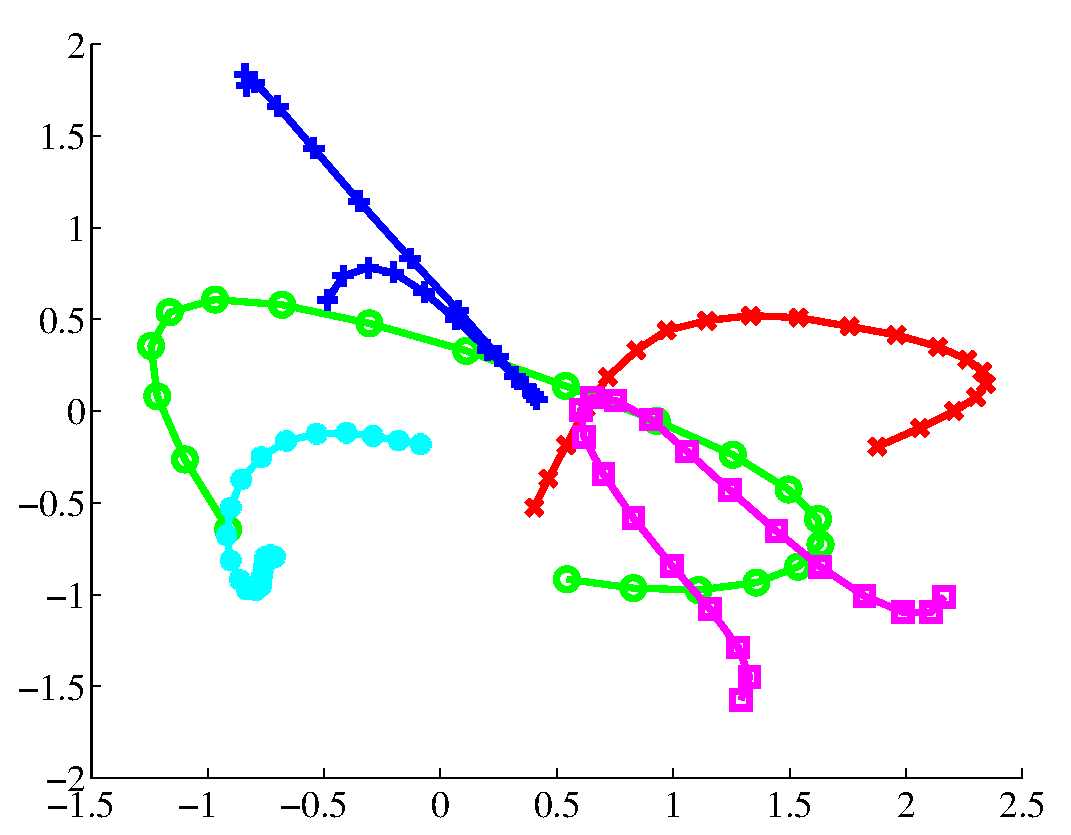
\includegraphics[width=0.8\columnwidth]{\lyxdot \lyxdot /diagrams/demTemporalSamplePaths}\par\end{centering}


\caption{Typical sample paths for the RBF covariance function as temporal
prior over the latent space.\label{fig:Typical-sample-paths}}
\end{figure}
 

The temporal prior in (\ref{eq:gpTemporalPrior}) can be combined
with the GP-LVM likelihood in (\ref{eq:gplvmLikelihood}) to form
a new model,\[
p\left(\mathbf{Y}|\mathbf{t}\right)=\int p\left(\mathbf{Y}|\mathbf{X}\right)p\left(\mathbf{X}|\mbox{\textbf{t}}\right)\mbox{d}\mathbf{X},\]
unfortunately such a marginalisation is intractable. Instead, we seek
to make progress by seeking a \emph{maximum a posteriori} (MAP) solution,
maximising\[
\log p\left(\mathbf{X}|\mathbf{Y},\mathbf{t}\right)=\log p\left(\mathbf{Y}|\mathbf{X}\right)+\log p\left(\mathbf{X}|\mathbf{t}\right)+\mbox{const.}\]
with respect to $\mathbf{X}$. The first term in this equation is
the standard objective function for the GP-LVM, the second term has
the form\[
\log p\left(\mathbf{X}|\mathbf{t}\right)=-\frac{1}{2}\prod_{j=1}^{q}\mathbf{x}_{:,j}^{\mbox{T}}\mathbf{K}_{t}^{-1}\mathbf{x}_{:,j}+\mbox{const.},\]
where $\mathbf{x}_{:,j}$ is the $j$th column of $\mathbf{X}$. The
gradient of this additional term may also be found,\[
\frac{\mbox{d}\log p\left(\mathbf{X}|\mathbf{t}\right)}{\mbox{d}\mathbf{X}}=\mathbf{K}_{t}^{-1}\mathbf{X}\]
and combined with the gradient of $\log p\left(\mathbf{Y}|\mathbf{X}\right)$
to find the MAP solution. This can easily be found using gradient
based methods.


\section{More Complex Hierarchies\label{sec:complexHierarchies}}

We now turn to a slightly more complex hierarchy than the dynamical
model described in the previous section. Consider a motion capture
example with multiple subjects interacting. Given the form of the
interaction it should be possible to model each subject independently.
This form of conditional independence is well captured by a hierarchical
model such as that shown in Figure~\ref{fig:twoSubjects}. 

%
\begin{figure}
\begin{centering}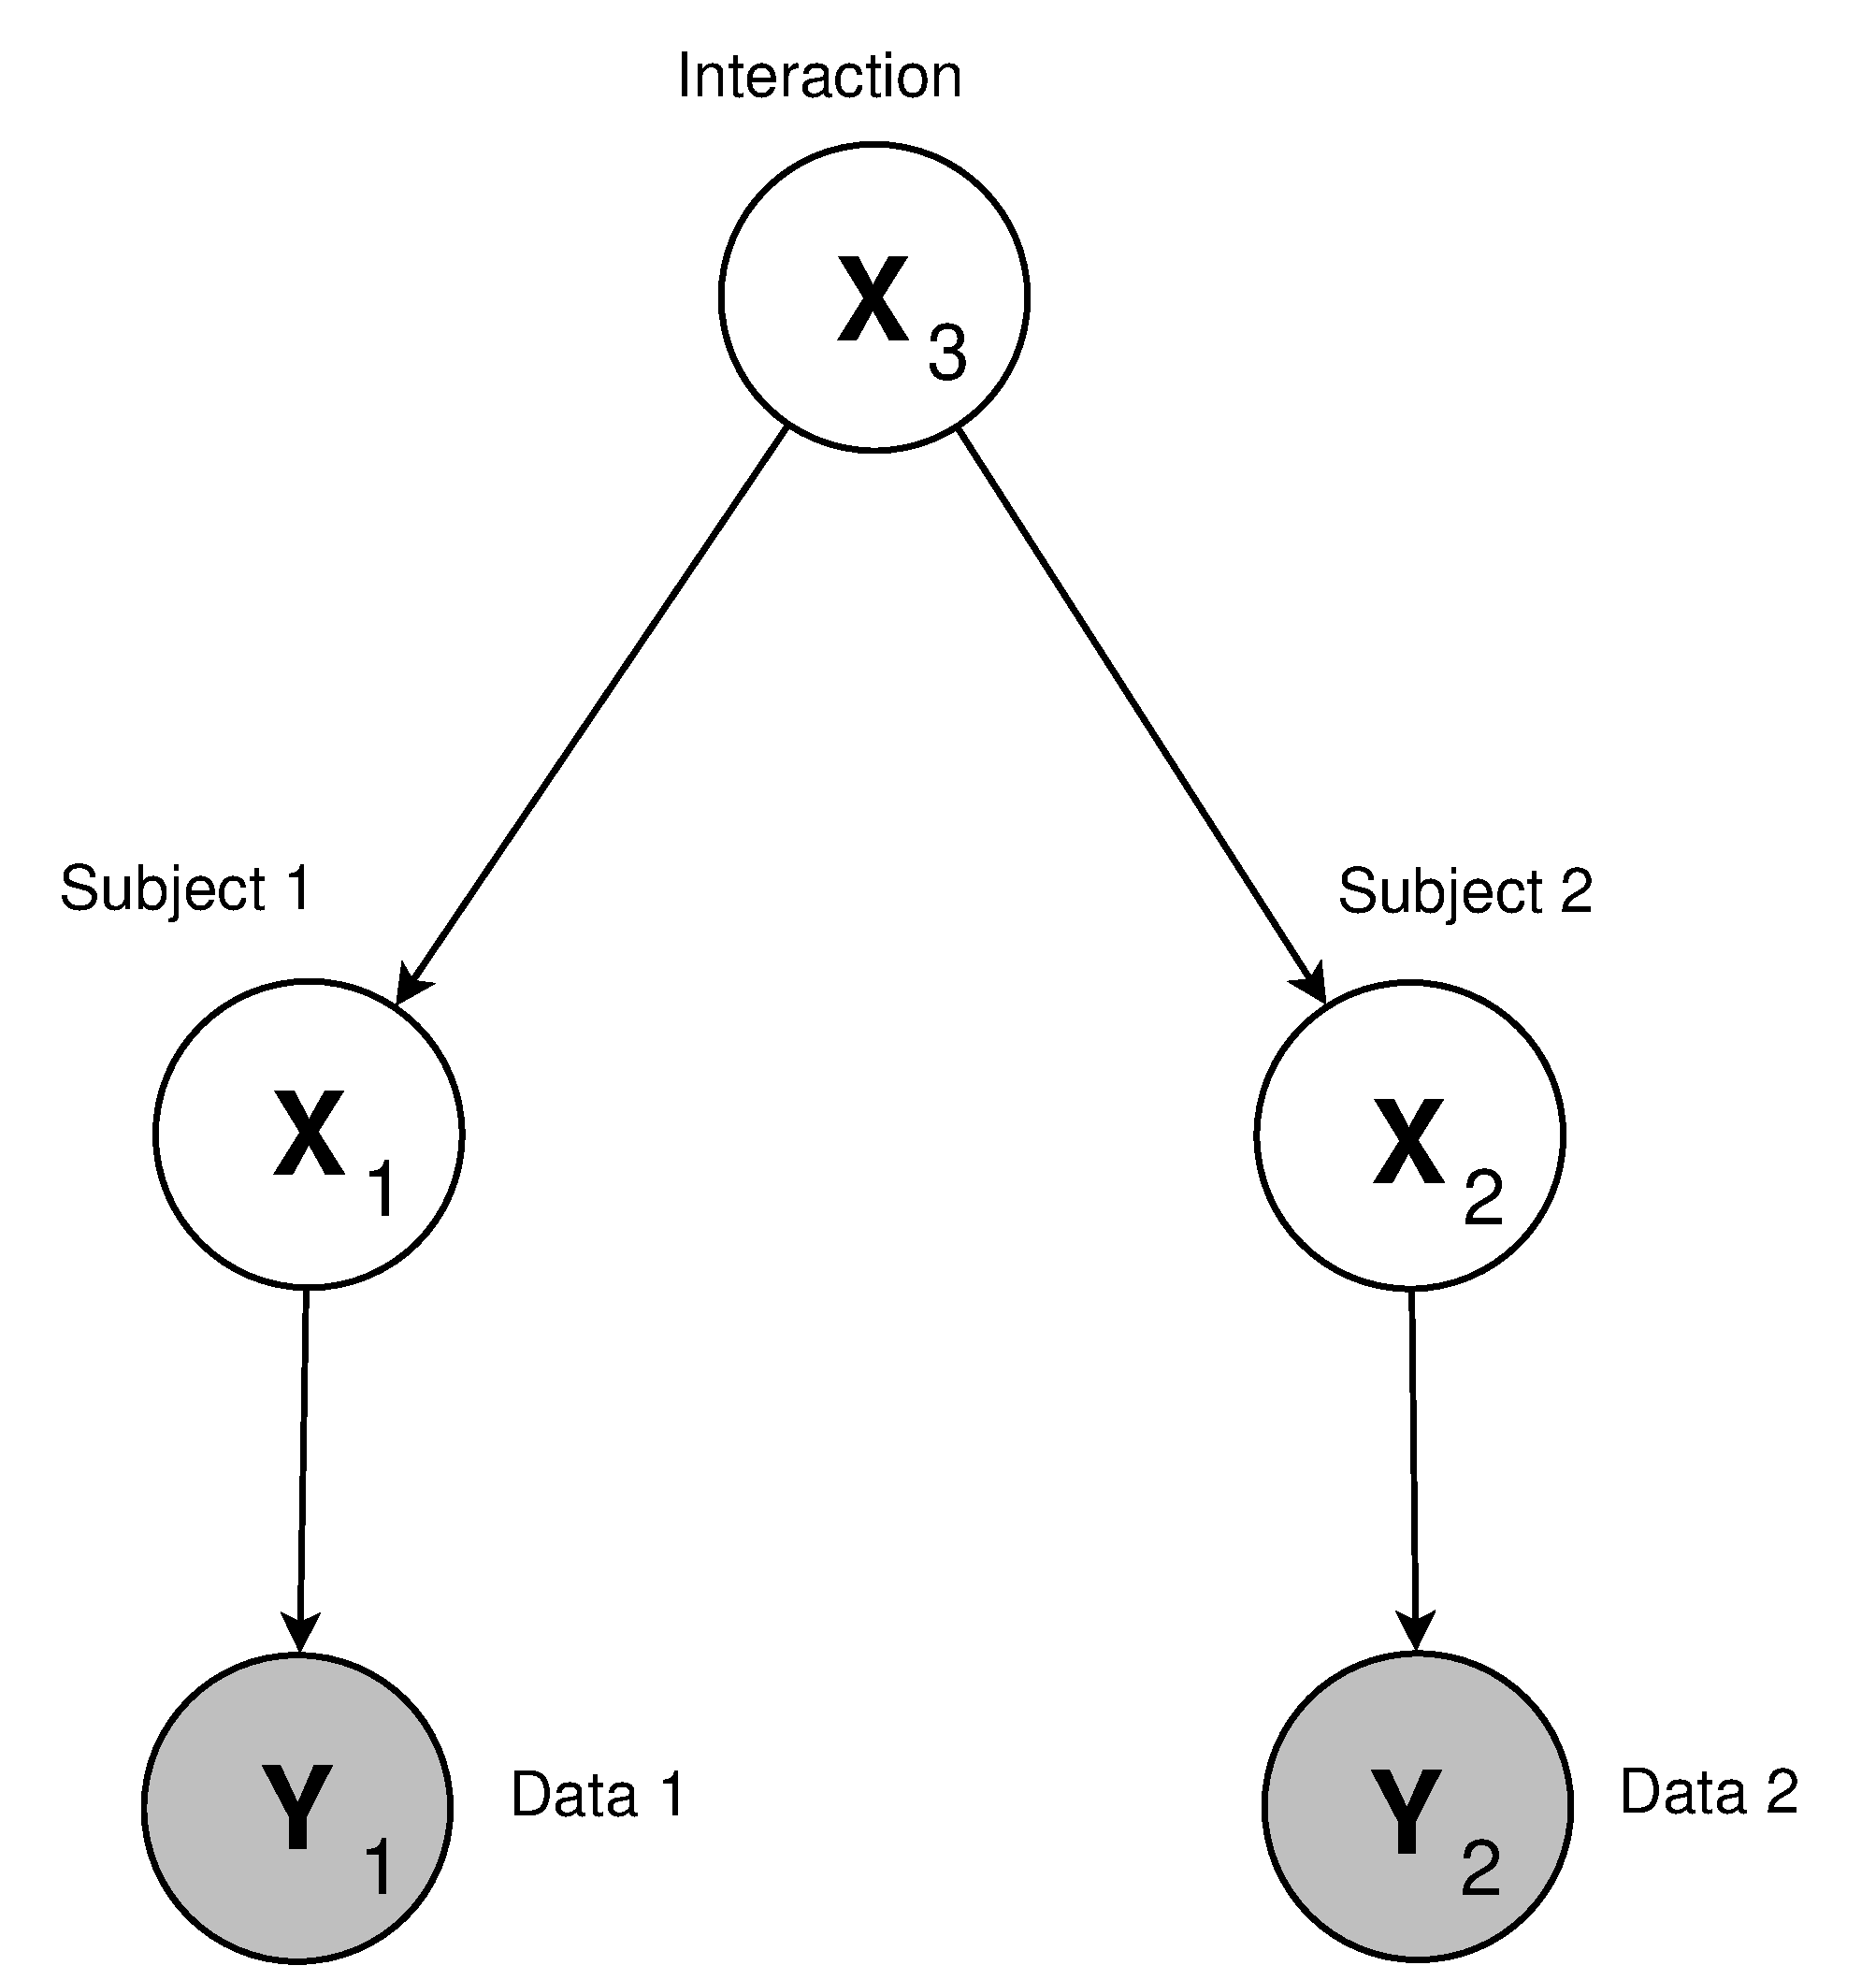
\includegraphics[width=0.7\columnwidth]{\lyxdot \lyxdot /diagrams/twoSubjects}\par\end{centering}


\caption{A simple hierarchy for capturing interaction between two subjects
where $\mathbf{Y}_{1}$ is the data associated with subject 1, $\mathbf{Y}_{2}$
is that of subject 2. Each of these variable sets is then controlled
by latent variables, $\mathbf{X}_{1}$ and $\mathbf{X}_{2}$. These
latent variables are in turn controlled by $\mathbf{X}_{3}$. \label{fig:twoSubjects}}
\end{figure}
The joint probability distribution represented by this graph is given
by\begin{eqnarray*}
p\left(\mathbf{Y}_{1},\mathbf{Y}_{2}\right) & = & \int p\left(\mathbf{Y}_{1}|\mathbf{X}_{1}\right)\dots\\
 &  & \times\int p\left(\mathbf{Y}_{2}|\mathbf{X}_{2}\right)\dots\\
 &  & \times\int p\left(\mathbf{X}_{1},\mathbf{X}_{2}|\mathbf{X}_{3}\right)\mbox{d}\mathbf{X}_{3}\mbox{d}\mathbf{X}_{2}\mbox{d}\mathbf{X}_{1}\\
 &  & ,\end{eqnarray*}
where each conditional distribution is given by a Gaussian process.
However, once again, the required marginalisations are not tractable.
We therefore turn to MAP solutions for finding the values of the latent
variables. For this model, this means maximisation of\begin{eqnarray*}
\log p\left(\mathbf{X}_{1},\mathbf{X}_{2}\mathbf{X}_{3}|\mathbf{Y}_{1},\mathbf{Y}_{2}\right) & = & \log p\left(\mathbf{Y}_{1}|\mathbf{X}_{1}\right)\\
 &  & +\log p\left(\mathbf{Y}_{2}|\mathbf{X}_{2}\right)\\
 &  & +\log p\left(\mathbf{X}_{1},\mathbf{X}_{2}|\mathbf{X}_{3}\right),\end{eqnarray*}
which is the sum of three Gaussian process log likelihoods. The first
two terms are associated with the two subjects. The third term provides
co-ordination between the subjects. 


\subsection{Two Interacting Subjects}

To demonstrate this hierarchical model we considered a motion capture
data set consisting of two interacting subjects. The data, which was
taken from the CMU MOCAP data base%
\footnote{\url{http://mocap.cs.cmu.edu}.%
}, consists of two subjects%
\footnote{The subjects used are numbered 20 and 21 in the data base. The motion
is number 11. %
} that approach each other and `high five'. 

The algorithm for optimisation of the latent variables proceeded as
follows:

\begin{enumerate}
\item Initialise each leaf node's latent variable set ($\mathbf{X}_{1},\mathbf{X}_{2}$)
through principal component analysis of the corresponding data set
($\mathbf{Y}_{1}$,$\mathbf{Y}_{2}$).
\item Initialise the root node's latent variable set ($\mathbf{X}_{3}$)
through principal component analysis of the concatenated latent variables
of its dependents $\left[\mathbf{X}_{1}\,\,\mathbf{X}_{2}\right]$.
\item Optimise jointly the parameters of the kernel matrices for each Gaussian
process model and the latent variable positions $\left(\mathbf{X}_{1},\mathbf{X}_{2},\mathbf{X}_{3}\right)$. 
\end{enumerate}
The original data is sampled at 120 frames per second. We extracted
frames 50 to 113, sub-sampling to 30 frames per second, frames 114
to 155 at the full sample rate and frames 156 to 232 sub-sampling
at 30 frames per second. This gives a data set with a variable sample
rate. In the context of this data the variable sample rate is important:
the section where we used the higher sample rate contains the slapping
of the two subjects hands. This motion is rapid and cannot be accurately
reconstructed with a sample rate of 30 frames per second. This variable
sample rate presents problems for the autoregressive dynamics we reviewed
in Section~\ref{sub:gaussianProcessDynamics}. However, for the regressive
dynamics we introduced in Section~\ref{sub:regressiveDynamics} the
variable sample rate can simply be reflected in the vector $\mathbf{t}$.
We therefore made use of these dynamics by adding a further layer
to the hierarchy,

\begin{eqnarray*}
p\left(\mathbf{Y}_{1},\mathbf{Y}_{2}|\mathbf{t}\right) & = & \int p\left(\mathbf{Y}_{1}|\mathbf{X}_{1}\right)\dots\\
 &  & \times\int p\left(\mathbf{Y}_{2}|\mathbf{X}_{2}\right)\int p\left(\mathbf{X}_{1},\mathbf{X}_{2}|\mathbf{X}_{3}\right)\dots\\
 &  & \times p\left(\mathbf{X}_{3}|\mathbf{t}\right)\mbox{d}\mathbf{X}_{3}\mbox{d}\mathbf{X}_{2}\mbox{d}\mathbf{X}_{1}.\end{eqnarray*}
However, we do not optimise the parameters of the dynamics: we wish
the latent space to be constrained by the dynamics. Finally, we would
like the effect of the dynamics to be present as we descend the the
hierarchy. To this end, we constrained the noise parameter, $\sigma_{\mbox{white}}^{2}$
of the Gaussian process associated with $p\left(\mathbf{X}_{1},\mathbf{X}_{2}|\mathbf{X}_{3}\right)$
to $1\times10^{-6}$. If we allow this variance to be free, the effect
of the dynamics could become diluted as we drop down the hierarchy.
By constraining this variance we force the temporal correlations present
in the data to be respected.

In Figure~\ref{fig:highFive} we show the results of mapping these
motions into this hierarchical model.

%
\begin{figure*}[t]
\begin{centering}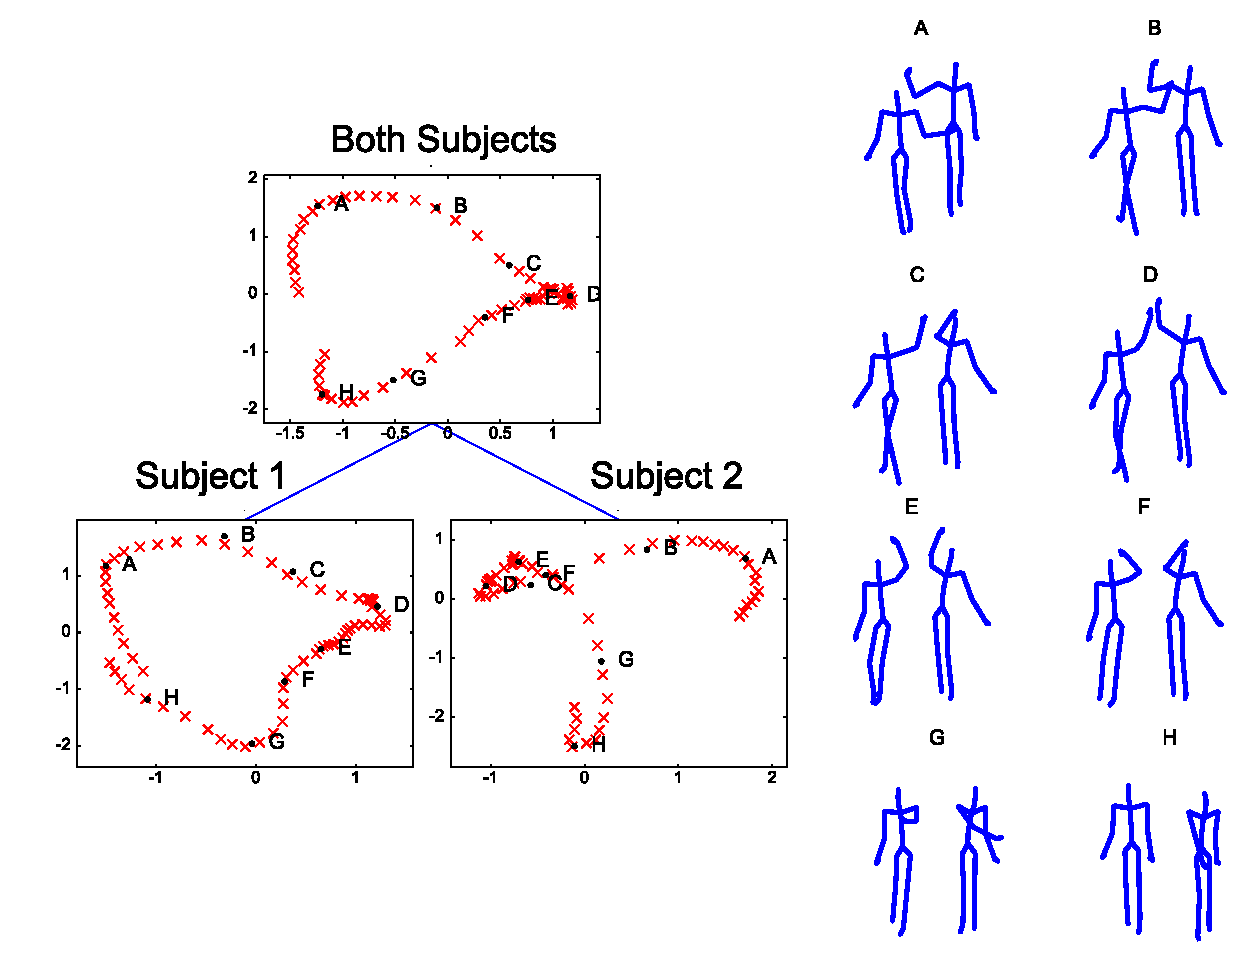
\includegraphics[width=0.7\textwidth]{\lyxdot \lyxdot /diagrams/demHighFive_talk}\par\end{centering}


\caption{High Five example. Two subjects are modelled as they walk towards
each other and `high five'. The plot shows the simple hierarchy used
to model the data. There is a regressive dynamical prior of the type
described in Section~\ref{eq:gpTemporalPrior} placed over the latent
space of the root node. The root node then controls the two individual
subjects. To illustrate the model we have taken points at time (i.e
we input these values of $t$ into the dynamical model) frames A:
85, B: 114, C:127, D: 141, E: 155, F: 170, G: 190 and H: 215. These
points mapped down through the hierarchy and into the data space.
In each of the plots of the two subjects, Subject 1 is on the right
and Subject 2 is on the left. \label{fig:highFive}}
\end{figure*}



\section{Subject Decomposition}

As well as decomposing the interactions between two subjects into
a hierarchy, we can also consider decomposition of a single subject
into parts. As we discussed in the introduction, there have been several
different approaches to modelling motion capture data through tree
based models, but these models typically assume that the nodes of
the tree are observed and that the tree rigidly reflects the skeletal
structure. Some effort has been made to model additional correlations
in motion data by augmenting the tree with an additional, common,
latent variable \cite{Lan:beyond05}. However, our hierarchical model
is closer in structure to the tree models of \cite{Williams:tree98}
where the tree structure refers to a \emph{hierarchy of latent variables},
rather than a hierarchy of the observed variables. 

%
\begin{figure}
\begin{centering}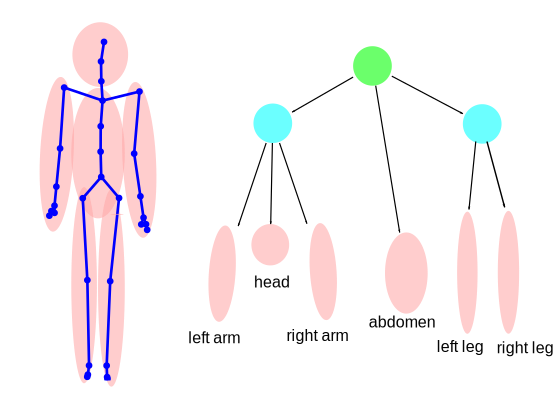
\includegraphics[width=0.9\columnwidth]{\lyxdot \lyxdot /diagrams/stickHierarchy}\par\end{centering}


\caption{Decomposition of skeleton for hierarchical modelling. By separating
the component parts of the skeleton in this manner we can model the
space of natural motions for each component part and express them
independently or jointly.\label{fig:skeletonDecomposition}}
\end{figure}


We considered a data set composed of a walking motion and a running
motion, again taken from the CMU MOCAP data base. The run was taken
from motion 25 of subject 35 and the walk was taken from motion 01
of subject 35. The data was sub-sampled to 30 frames per second and
one cycle of each motion was used. The x and y location of each motion's
`root position' was set to zero so that the subject was running/walking
`in place'. We modelled the subject using the decomposition shown
in Figure~\ref{fig:skeletonDecomposition}, but to reflect the fact
that two different motions were present in the data we constructed
a hierarchy with \emph{two roots}. One root was associated with the
run and a second root was associated with the walk. The prior induced
by the run root was applied only to the run data points in the next
layer of the hierarchy (abdomen, legs, upper body). Similarly, the
prior induced by the walk root was applied only to data points from
the walk data. The upper body, legs and all the leaf nodes were applied
to the entire data set. This construction enables us to express the
two motion sequences separately whilst retaining the information required
to jointly model the component parts of the skeleton. The aim is for
nodes in the lower levels of the hierarchy to span the range of motions,
whilst the upper layer specifies the particular motion type.

%
\begin{figure*}
\begin{centering}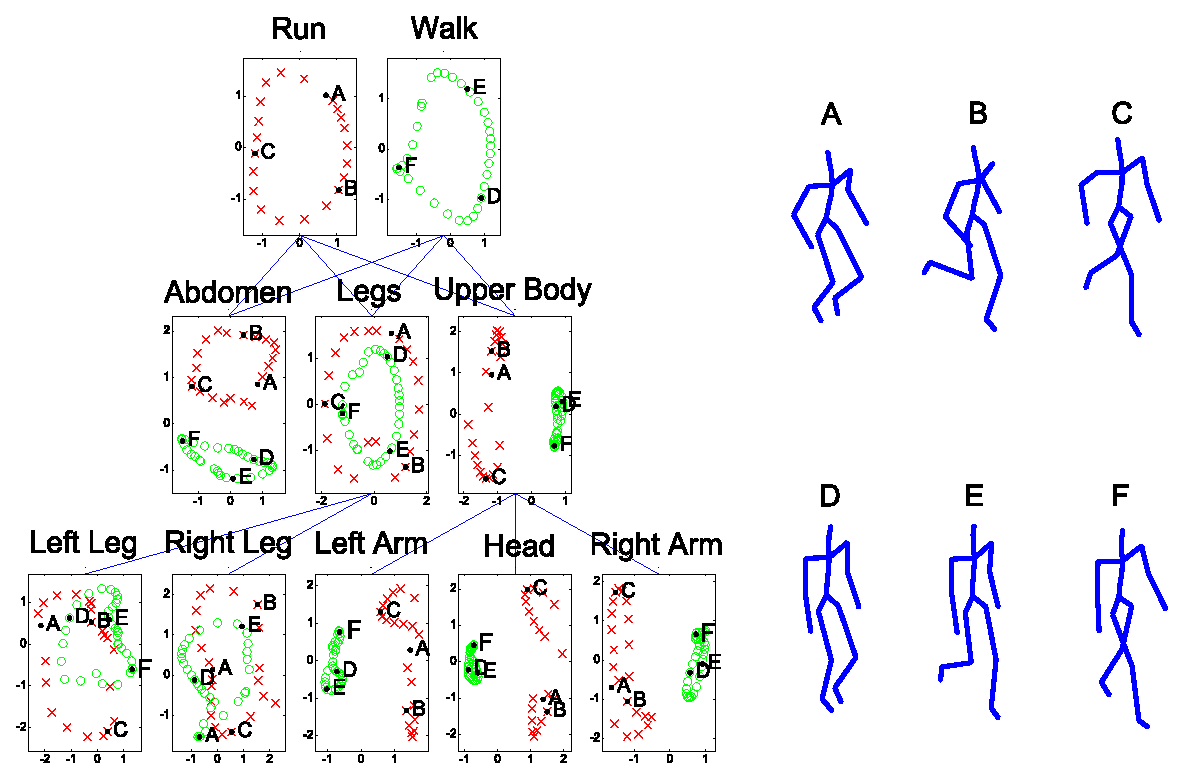
\includegraphics[width=0.7\textwidth]{\lyxdot \lyxdot /diagrams/demWalkRun_talk}\par\end{centering}


\caption{Combined model of a run and a walk. The skeleton is decomposed as
shown in Figure~\ref{fig:skeletonDecomposition}. In the plots, crosses
are latent positions associated with the run and circles are associated
with the walk. We have mapped three points from each motion through
the hierarchy. Periodic dynamics was used in the latent spaces.\label{fig:demRunWalk1}}
\end{figure*}


As the motion is broadly periodic, we made use of a periodic kernel
\cite{MacKay:gpintroduction98} for the regressive dynamics in each
latent space (see pg. 92 in \cite{Rasmussen:book06} for details).
The resulting visualisation is shown in Figure~\ref{fig:demRunWalk1}.


\section{Discussion}

We have presented a hierarchical version of the Gaussian process latent
variable model. The Gaussian process latent variable model involves
a paradigm shift in probabilistic latent variable models where, rather
than marginalising the latent variables and optimising the mappings,
we marginalise the mappings and optimise the latent variables. This
makes far easier to construct hierarchies of these models. The philosophy
of optimising versus marginalising is carried through to the hierarchical
GP-LVM: we maximise with respect to all the latent variables in the
different levels of the hierarchy.


\subsection{Overfitting}

Modelling with the GP-LVM is characterised by the use of very large
numbers of `parameters' in the form of the latent points. In the standard
case, the number of parameters increases linearly as a fraction, $\frac{q}{d}$,
of the number of data. As long as $q<d$ (how much less depends on
the data set) problems of overfitting do not normally occur. However,
we are now adding additional latent variables, do we not now run the
risk of overfitting the data if the hierarchy becomes too deep? The
first point to note is that the upper levels of the hierarchy only
serve to regularise the leaf nodes: so if the leaf nodes independently
do not overfit, neither will the entire model. In other words, we
must ensure that the leaf nodes each have $q_{i}<d_{i}$ where $q_{i}$
is the number of columns of $\mathbf{X}_{i}$ and $d_{i}$ is the
dimensionality of $\mathbf{Y}_{i}$. However, by modifying the locations
of latent variables in nodes higher up the hierarchy we are changing
the nature of the \emph{regularisation} of the leaf nodes. If unconstrained
the model could simply act in such a way as to remove the regularisation.
In our implementation we attempted to counter this potential problem
in two ways. Firstly, we provided a fixed dynamical prior at the top
level. The parameters of this prior were not optimised, so the top
level node is always `regularised%
\footnote{The same goal could also be achieved through \emph{back constraints}
\cite{Lawrence:backconstraints06}, but we did not explore that approach
here.%
}'. However, there is the possibility that this fixed regularisation
could be `diluted' by noise as we descend the hierarchy. To prevent
this happening we constrained the noise variance of each Gaussian
process that was not in a leaf node to $1\times10^{-6}$, \emph{i.e.}
close to zero but high enough to prevent numerical instabilities in
kernel matrix inverses. This strategy proved effective in all our
experiments.


\subsection{Other Hierarchical Models}

Given apparent similarities between the model names, it is natural
to ask what is the relationship between the hierarchical GP-LVM and
the hierarchical probabilistic PCA of \cite{Bishop:hierarchy98}?
The two models are philosophically distinct. In hierarchical PCA (and
the related hierarchical GTM model of \cite{Tino:hierarchical02})
every node in the hierarchy is associated with a probabilistic model
in \emph{data space}. The hierarchy is not a hierarchy of latent variables,
it is, instead, a hierarchical clustering of mixture components in
a discrete mixture of probabilistic PCA models (or GTM models). A
similar approach could be taken with the GP-LVM, but it is not the
approach we have described here.


\subsection{Applications}

We see the hierarchical GP-LVM as an important tool in several application
areas. However, there are two application areas in which we believe
the algorithm has particular promise. Firstly, the GP-LVM has already
been proposed as a prior model for tracking. A key problem with constructing
such prior models is that it is difficult to cover the space of all
natural human motions. However, using the hierarchical model we expect,
inspired by language modelling, to be able to perform a variant of
`back off'. Depending on motion, different models could be swapped
in at the top level of the hierarchy, however some actions will still
not be well modelled. In this case we suggest `backing off', which
in this context would translate into dropping down the hierarchy and
applying the models in the next layer of the hierarchy \emph{independently}
to the data. Another application area where we see great promise for
the model is animation. Through the hierarchical GP-LVM model different
portions of the a character can be animated separately or jointly
as circumstances demand. Animator time is becoming a dominating cost
in both the games and film entertainment industries where computer
special effect techniques are used, through combination of the hierarchical
GP-LVM with appropriate inverse kinematic techniques \cite{Grochow:styleik04}
we could seek to ameliorate these costs.


\subsection*{Acknowledgements}

This work was funded by the EU FP6 PASCAL Network of Excellence under
a pump priming grant. The motion capture data used in this project
was obtained from \texttt{mocap.cs.cmu.edu}. The database was created
with funding from NSF EIA-0196217. We thank Raquel Urtasun for helpful
discussions.

\appendix

\section{Recreating the Experiments}

The source code for re-running all the experiments detailed here is
available from \url{http://www.cs.man.ac.uk/~neill/hgplvm/}, release
0.1. 

\bibliographystyle{mlapa}
\bibliography{lawrence,other,zbooks}

\end{document}
